\documentclass[11pt]{article}
\usepackage[margin=1.1in]{geometry}
\usepackage{amsmath,amssymb,amsthm}
\usepackage{graphicx}
\usepackage{booktabs}
\usepackage{xcolor}
\usepackage[colorlinks=true,linkcolor=blue!50!black,citecolor=blue!50!black,urlcolor=blue!50!black]{hyperref}
\graphicspath{{outputs/}}

\newtheorem{prop}{Proposition}
\newtheorem*{remark}{Remark}

\newcommand{\Jpm}{J_{\pm}}
\newcommand{\Jzz}{J_{zz}}
\newcommand{\btheta}{\boldsymbol{\theta}}
\newcommand{\bq}{\mathbf{q}}
\newcommand{\bw}{\mathbf{w}}
\newcommand{\avg}[1]{\left\langle #1 \right\rangle}
\newcommand{\Z}{\mathbb{Z}}

\title{Why observable-level twist averaging cannot remove\\ the winding artifact
--- and where it would work}
\author{\texttt{twist\_qsi\_demo} campaign note}
\date{July 2026}

\begin{document}
\maketitle

\noindent\emph{Companion note to \texttt{run\_twist\_average.py},
\texttt{src/qsi\_campaign/twist\_average.py}, and
\texttt{outputs/fig\_twist\_average.pdf} (data:
\texttt{outputs/twist\_average\_scan\_m\{1,2,3\}.json}; spectra cached in
\texttt{cache/twist\_avg/}).  Every number below is an exact-diagonalization
result on the cubic 16-site cluster, reproducible from those scripts.}

\section{The object to be removed}

On a torus one unit cell across, the shortest ice-preserving loop that wraps
the boundary has \emph{four} sites, while the shortest contractible loop ---
the hexagon carrying the physical ring exchange --- has \emph{six}.
Degenerate perturbation theory therefore produces the wrapping process at
second order,
\begin{equation}
  g_4 = \frac{4\Jpm^2}{\Jzz},
\end{equation}
parametrically \emph{above} the physical third-order scale
\begin{equation}
  g_6 = \frac{12\,|\Jpm|^3}{\Jzz^2}.
\end{equation}
The low-temperature heat-capacity peak of the bare periodic cluster sits on
the $g_4$ scale: it is an artifact of processes that exist only because the
torus is small.  Each such process is labelled by its homology winding
$\bw\in\Z^3$; the census on cubic-16 is given in
Table~\ref{tab:census}.  Locally these processes are legitimate ice dynamics
--- the winding label is the \emph{only} thing wrong with them, so any cure
must act on that topological label and on nothing else.

\begin{table}[h]
\centering
\begin{tabular}{lcccc}
\toprule
PT order & wrapping loops & winding pattern & $\sum_i w_i$ even & $\sum_i w_i$ odd\\
\midrule
2 (4-loops) & 36 & $24\times(\pm\mathbf{e}_i)$,\; $12\times(\mathbf{e}_i\pm\mathbf{e}_j)$ & 12 & 24\\
3 (6-loops) & 80 & $48\times(\mathbf{e}_i\pm\mathbf{e}_j)$,\; $32\times(\mathbf{e}_x\pm\mathbf{e}_y\pm\mathbf{e}_z)$ & 48 & 32\\
\bottomrule
\end{tabular}
\caption{Winding-loop census of the cubic 16-site cluster by perturbative
order.  The even/odd split of the component sum controls which loops any
single twist can annihilate (Sec.~\ref{sec:walls}).}
\label{tab:census}
\end{table}

\section{What a twist actually does to a winding process}
\label{sec:twist}

Work in the smooth (translationally invariant) gauge: every $S^+_iS^-_j$ hop
carries $e^{2i\btheta\cdot\mathbf{d}_{ij}}$, with $\mathbf{d}_{ij}$ the lifted
bond displacement.  Because the ice manifold is an emergent-charge-free
vacuum, a \emph{completed} ice-to-ice process is sensitive only to the total
$S^z$ dipole it transports, and for a loop that dipole is pure topology,
\begin{equation}
  \boldsymbol{\rho} = \tfrac12\,\bw L
\end{equation}
(verified exactly for all $84+120$ winding loops of the cubic and FCC
clusters).  Three consequences, each verified numerically to machine
precision in this campaign:
\begin{enumerate}
\item \textbf{Contractible loops transport nothing} ($\boldsymbol{\rho}=0$):
  the hexagon amplitude is twist-independent.  No twist can touch the physics.
\item \textbf{Matched-pair interference.}  The two virtual orderings of a
  winding ring exchange transport the dipole in \emph{opposite} half-cell
  senses ($\pm\boldsymbol{\rho}$), so their smooth-gauge phases interfere
  \emph{within a single Hamiltonian}:
  \begin{equation}
    c(\btheta) \;=\; g\,\cos(\btheta\cdot\bq),
    \qquad \bq \equiv 2\boldsymbol{\rho} = \bw L \in \Z^3 .
    \label{eq:cosine}
  \end{equation}
  This is genuine destructive interference between virtual paths: the
  amplitude vanishes identically when $\btheta\cdot\bq = \pi/2 \pmod{\pi}$.
\item \textbf{Corner twists are pure gauge.}  At
  $\btheta\in\{0,\pi\}^3$ the cosine is $\pm1$, and a sign on an off-diagonal
  matrix element is removed by the diagonal unitary
  $V(\btheta)=e^{2i\btheta\cdot X}$, $X=\sum_i \mathbf{r}_i S^z_i$.  Verified
  at the full $65{,}536$-state microscopic level: the corner spectrum equals
  the periodic spectrum to $4\times10^{-14}$.  \emph{The all-$\pi$ twist does
  exactly nothing.}
\end{enumerate}
The hoped-for interference therefore exists --- but as a cosine of the single
projection $\btheta\cdot\bq$, not as a switch that can be thrown for all
$\bq$ at once.

\section{The two walls}
\label{sec:walls}

\paragraph{Wall 1: observables average probabilities, not amplitudes.}
In the solve-per-twist scheme each twist is an independent exact Hamiltonian.
Its spectrum is gauge invariant and feels the winding amplitude only through
$|c(\btheta)|^2 \propto \cos^2(\btheta\cdot\bq)$.  Averaging $C(T)$ over
twists therefore adds \emph{weights}: phases belonging to different twists
never sit in the same matrix element and cannot cancel.  The uniform torus
average leaves every winding loop with
\begin{equation}
  \avg{\cos^2(\btheta\cdot\bq)}_{\btheta} = \tfrac12
\end{equation}
--- half the contamination power, at every coupling, forever.

\paragraph{Wall 2: direction frustration.}
Amplitude-level killing by a single twist demands
$\btheta\cdot\bq \equiv \pi/2 \pmod{\pi}$ for \emph{every} winding vector in
the census simultaneously.  The 24 axis loops require
$\theta_i \equiv \pi/2 \pmod{\pi}$ for all three axes; that forces
$\theta_i\pm\theta_j \equiv 0 \pmod{\pi}$ --- exactly the wrong value for the
12 diagonal loops $\bw=\mathbf{e}_i\pm\mathbf{e}_j$.  The best any single
twist can achieve is
\begin{equation}
  \min_{\btheta}\;\sum_{\text{loops}}\cos^2(\btheta\cdot\bq)
  \;=\; \frac{12}{36} \;=\; \frac13,
\end{equation}
attained at $\btheta=(\pi/2,\pi/2,\pi/2)$: every odd-parity loop annihilated
exactly, every even-parity loop at \emph{full} strength.  Table~\ref{tab:census}
shows the same split at third order (48 of the 80 wrapping hexagons are
even), so the surviving sector is not a low-order accident: even-winding
processes survive \emph{any} phase assignment at \emph{any} order, since
$\cos(\text{even}\cdot\pi/2)=\pm1$.

\begin{prop}[Observable-level floor]
The surviving winding weight of any twist-ensemble average with probability
measure $\mu$,
\begin{equation}
  W[\mu] \;=\; \sum_{\text{loops}} \int \! d\mu(\btheta)\,
  \cos^2(\btheta\cdot\bq),
\end{equation}
is linear in $\mu$; its minimum over all probability measures is attained by
a point mass at the optimal single twist.  Hence on cubic-16
\begin{equation*}
  \underbrace{1}_{\text{bare}} \;>\;
  \underbrace{\tfrac12}_{\text{uniform average}} \;>\;
  \underbrace{\tfrac13}_{\text{optimal single twist }(\pi/2)^3} \;>\;
  \underbrace{0}_{\text{unreachable}} ,
\end{equation*}
and no observable-level twist scheme --- averaged, optimized, or otherwise ---
can do better than the single twist $(\pi/2,\pi/2,\pi/2)$.
\end{prop}

\section{What the measurement shows}

Table~\ref{tab:powerlaws} summarizes the 41-point $\Jpm$ scan
(full $65{,}536$-state spectra per twist per coupling; see
Fig.~\ref{fig:twist}).  Every observable-level twist scheme keeps the $g_4$
\emph{power law} and only shrinks its prefactor ($1 : 0.62 : 0.28$); only the
operator-level mask crosses over to $g_6$ scaling.  The twist protocols do
run through the entire dissolved regime ($\Jpm = -0.19$ to $-0.30$), where the
band construction fails; there the single twist is the cleanest tool, because
the averaged curve is a mixture whose maximum is grid fragile (at
$\Jpm=-0.25$ the $M{=}2$ average puts the peak at $0.051\,\Jzz$ but $M{=}3$ at
$0.086\,\Jzz$, agreeing with the single twist).

\begin{table}[h]
\centering
\begin{tabular}{lcc}
\toprule
protocol & $T_{\rm peak}$ scaling ($|\Jpm|\le 0.05$, $\pi$ flux) &
$T_{\rm peak}/\Jzz$ at $\Jpm=-0.05$\\
\midrule
bare periodic ED           & $|\Jpm|^{1.77}$ & $0.0130$\\
uniform twist average      & $|\Jpm|^{1.76}$ & $0.0080$\\
single twist $(\pi/2)^3$   & $|\Jpm|^{1.80}$ & $0.0037$\\
winding-free mask          & $|\Jpm|^{2.86}$ & $0.0012$\\
\bottomrule
\end{tabular}
\caption{Measured lower-peak position: power-law fits and representative
values.  The twist family reduces the artifact prefactor by at most a factor
$\sim3$ and never changes the $g_4$-like exponent; the mask alone reaches the
physical $g_6$ scaling.}
\label{tab:powerlaws}
\end{table}

\begin{figure}[h]
\centering
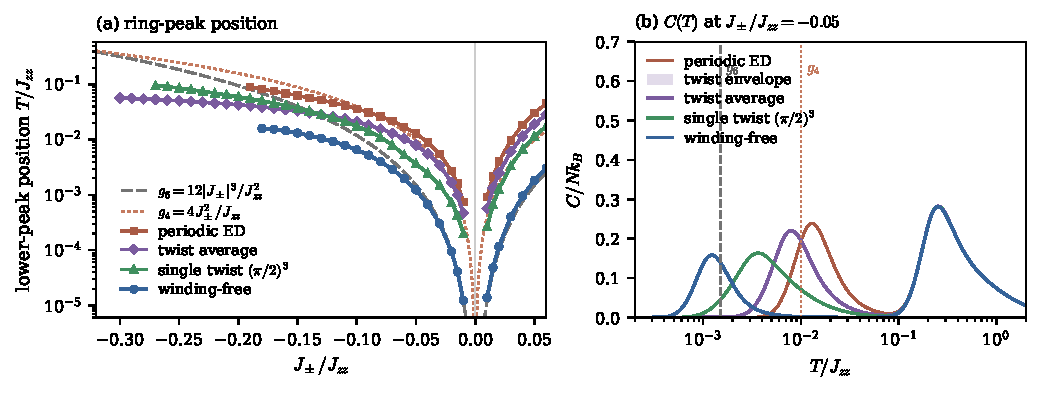
\includegraphics[width=\textwidth]{fig_twist_average}
\caption{(a) Lower-peak position across the $\Jpm$ scan for the four
protocols against the perturbative scales $g_4$ and $g_6$.  (b) $C(T)$ at
$\Jpm/\Jzz=-0.05$: the twist envelope shows the spread of the individual
twisted spectra entering the average; the spinon peak at $T\sim\Jzz/4$ is
identical in all protocols.}
\label{fig:twist}
\end{figure}

\section{Why the mask escapes both walls}

The winding-free protocol averages the \emph{operator} over the character
grid before diagonalizing,
\begin{equation}
  H_{\rm clean} \;=\;
  \avg{V(\btheta)\, H_{\rm band}(0)\, V(\btheta)^\dagger}_{\btheta\,\in\,\text{corners}},
  \qquad
  \avg{e^{-i\btheta\cdot\bq}}_{\btheta} = \delta_{\bq,\mathbf{0}} .
\end{equation}
That average is coherent --- it acts on amplitudes, deleting every winding
matrix element identically, at all orders, with no direction compromise (at
$M{=}2$ it is the polarization-parity mask of Theorem~B).  It escapes Wall~1
by acting \emph{before} the nonlinearity of diagonalization, and Wall~2
because character projection uses the full group average rather than one
phase point.  Homotopy fixes the price: $T^3=K(\Z^3,1)$ makes winding the
complete topological label, so this cleaning is maximal --- and it requires
the ice-descended band to exist, i.e.\ band isolation.

\section{Regimes where twist averaging \emph{does} work}

The failure is specific to \emph{topological tunnelling amplitudes probed
through gauge-invariant observables}.  Twist averaging is the right tool when
the boundary condition enters differently:
\begin{enumerate}
\item \textbf{Operator level, always.}  But that \emph{is} the winding-free
  mask: ``twist averaging done coherently'' and the production protocol are
  the same object.
\item \textbf{Dispersion sampling (Lin--Zong--Ceperley).}  When an observable
  depends on the twist through single-quasiparticle energies
  $\varepsilon(\mathbf{k}+\btheta/L)$ --- shell effects, not tunnelling ---
  the twist average literally performs the Brillouin-zone integral and
  genuinely accelerates convergence to the bulk.  Here that regime is the
  \emph{spinon continuum / high-temperature sector} ($T\sim\Jzz$), which
  lives outside the ice manifold, carries no winding contamination, and is
  where the simulation plan already uses the twist grid legitimately (FTLM
  $S(\mathbf{q},\omega)$ interpolation).
\item \textbf{Clusters where winding is subleading.}  On a torus at least two
  unit cells across in every direction, the shortest winding loop is longer
  than the hexagon, the artifact appears beyond order six, and the
  unremovable $\tfrac13$--$\tfrac12$ residual multiplies something already
  parametrically negligible.  (Not available here: cubic-16 \emph{and}
  FCC-32 both host winding 4-loops along their short cycles.)
\item \textbf{Censuses without the even-parity sector.}  If a cluster's
  winding vectors all had odd component sum, $(\pi/2)^3$ would annihilate the
  entire leading artifact in amplitude.  Cubic-16 fails this (12 even
  4-loops), and even-parity windings reappear at higher order regardless ---
  a geometric accident, not a strategy.
\end{enumerate}

\begin{remark}
The dichotomy worth remembering: \emph{twist averaging fixes
$\mathbf{k}$-quantization errors; it cannot fix topological tunnelling
amplitudes}, because gauge-invariant observables see those only through their
magnitude.  For gauge-sector thermodynamics on ED-sized QSI tori,
observable-level twisting --- averaged or optimally chosen --- reduces the
winding artifact by at most a factor of three and never changes its power
law; complete removal requires phases to meet \emph{inside} matrix elements,
which only the operator-level character projection provides.
\end{remark}

\end{document}
